\documentclass[10pt,a4paper]{article}
\usepackage{amssymb,amsmath}
\usepackage{graphicx} 	 
\usepackage{times}
\title{Introduction To Vision And Robotics \\ Vision Assignment}
\author{Clemens Wolff, Toms Bergmanis}
\date{March 7th, 2013}

\begin{document}

\maketitle

\section{Introduction}
This report describes the work done for the first assignment in the IVR course. 
It gives the aims and hypotheses that guided the work; describes the algorithms 
that were implemented and reports the results of experiments that were run.
The goal of this assignment was to develop three algorithms: one that detects 
the robots in each image, one that correctly identifies the direction of the 
robot and one that links together detections of the robots in consecutive 
images. 
Several simplifying assumptions were made about the possible set-ups of the 
assignment.  Firstly, it was assumed that colours of the robots may change only 
due to the light it is exposed to, thus giving a rise to an assumption that 
robots will each appear in various shades of red or blue or green. Secondly, it 
was assumed that camera will be set up in some reasonable angle with respect to 
the plane it is supposed to observe. Finally, due to colour dependant approach 
it was assumed that background of the image will be in colour other than any of 
the colours of the robots.


\section{Methods}
In the following sections the three algorithms are described in detail. 

\subsection{Detection of Robots}
\begin{description}
\item[Input] \hfill \\
    $I$, a three channel image of dimensions m*n in the RGB colorspace.
\item[Output] \hfill \\
    $M$, a m*n*3 binary matrix where for each pixel $(i,j)$ of $I$, it holds 
    that: \\
    $M(i,j,1) = 1 \leftrightarrow (i,j)$ belongs to the red robot, \\
    $M(i,j,2) = 1 \leftrightarrow (i,j)$ belongs to the green robot, \\
    $M(i,j,3) = 1 \leftrightarrow (i,j)$ belongs to the blue robot.
\end{description}
\textbf{Algorithm}
\begin{enumerate}
    \item
    Apply approximate RGB-normalisation to $I$, giving $I_n$:
    \begin{itemize}
        \item
        For each pixel in $I_n$, calculate the sum S$_{rgb}$ of the red, green, 
        and blue values of that pixel.
        \item
        If the pixel is not absolute black (S$_{rgb}$ $\ne$ 0), set each of the 
        pixel's red, green, and blue values to that value divided by S$_{rgb}$.
    \end{itemize}

    \item
    Calculate $\mu_r, \mu_g, \mu_b$ and $\sigma_r, \sigma_g, \sigma_b$, the 
    means and standard deviations of the values in the three channels of $I_n$.

    \item
    Assign each pixel $P = (i,j)$ in $I$ to one of the robots or to the 
    background:
    \begin{itemize}
        \item
        Normalise $P$'s red, green, and blue values, giving $P_n$.
        \item
        Calculate the probabilities $p_r, p_g, p_b$ that $P_n$ was generated 
        by the gaussian distributions $\mathcal{N}_r = (\mu_r, \sigma_r),
        \mathcal{N}_g = (\mu_g, \sigma_g), \mathcal{N}_b = (\mu_b, \sigma_b)$.
        \item
        Calculate $P$'s hue value $h$.
        \item
        If $h$ is whithin a certain range defined as red and $p_r$ is
        sufficiently small, set $M(i,j,1) = 1$ (similarly for ranges defined as
        green/blue and $p_g$/$p_b$. If none of these conditions are met, set
        $M(i,j,1) = M(i,j,2) = M(i,j,3) = 0$.
    \end{itemize}

    \item
    Remove noise from each channel in $M$:
    \begin{itemize}
        \item
        Set pixels to zero if they have fewer neighbours with value one than
        they have adjacent pixels with value zero.
        \item
        Set zero-valued pixels to one if they have two one-valued 
        horizontal or vertical neighbours.
    \end{itemize}

    \item
    Remove components that are distant from the main concentration of mass in
    each channel in $M$:
    \begin{itemize}
        \item
        Compute the center of mass $C$ of the channel.
        \item
        Compute $c_1, c_2, \ldots$, the centers of mass of each connected 
        component in the channel.
        \item
        Compute the mean distance $C_m$ of the $c_k$ to $C$.
        \item
        Set $M(i,j) = 0$ for all the pixels $(i,j)$ in those components $i$ that
        have $c_i > t \cdot C_m$ for some threshold $t$.
    \end{itemize}

    \item
    Exploit the fact that all robots have similar sizes by setting every channel
    in $M$ to all-zeros if the number of pixels set in that channel is smaller
    than the number of pixels set in the most populated channel by some margin.

    \begin{figure}[h]
        \centering
        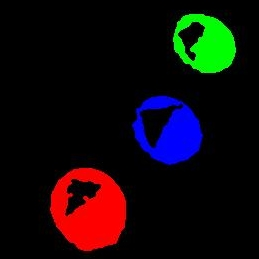
\includegraphics[width=40mm]{d1_i5_blob_mask.jpg}
        \caption{Result of Robot detection}
    \end{figure} 
\end{enumerate} 

\subsection{Detection of Directions}
\begin{enumerate}
    \item
    After having detected robot as a set of points in the image a convex hull 
    of these points was calculated.
    \textit{
    Further detection of the direction of the robot was done under the 
    assumption that colour representing the robot is different and appears 
    differently than that of the triangle indicating it's direction. 
    Furthermore - it was assumed that the triangle will have lesser pixel 
    colour value in the channel representing robot's colour (red or green, or 
    blue) in RGB representation than the average pixel of the convex hull. 
    These assumptions can be justified by the fact that area of the triangle 
    indicating the direction of the robot constituted relatively smaller area 
    of the convex hull than the rest of the convex hull which was expected to 
    appear in some other colour than black.
    } 

    \item
    The average pixel value of the characteristic channel was computed. Pixels 
    which were above that value were assigned to one mask, others were omitted 
    thus triangles were demasked.
    \begin{figure}[h]
        \centering
        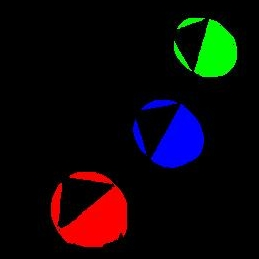
\includegraphics[width=40mm]{d1_i5_demasked_triangles.jpg}
        \caption{Demasked triangles (step 2)}
    \end{figure} 

    \item
    A convex hull of the result of step 2 was calculated.
    \textit{
    This step gives tighter and less noisy set of pixels that represent robot's
    coloured part in some harder cases.
    }

    \item
    A convex hull was computed for the result of the previous step. 

    \item
    Once more the average pixel value of the characteristic channel was 
    computed. This time pixels which were above that value were assigned to 
    one mask, others were assigned to another mask which was expected to 
    represent the triangle part of the robot's image.
    \begin{figure}[h]
        \centering
        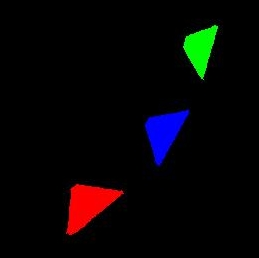
\includegraphics[width=40mm]{d1_i5_triangles.jpg}
        \caption{Triangles (step 5)}
    \end{figure} 

    \item
    Centres of both masks from the previous step were computed. 

    \item
    Then a line joining them was drawn which depending on how precisely robot
    was detected would correspond to the direction of the robot.
    \begin{figure}[h]
        \centering
        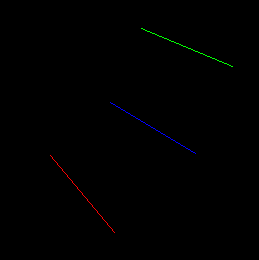
\includegraphics[width=40mm]{d1_i5_lines.png}
        \caption{Lines (step 7)}
    \end{figure} 

    \item
    Result was ploted on the source image.
    \begin{figure}[h]
        \centering
        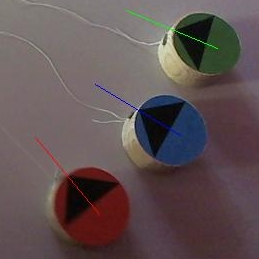
\includegraphics[width=40mm]{d1_i5_result.jpg}
        \caption{Result (step 8)}
    \end{figure} 
\end{enumerate} 

\subsection{Tracking of Robots}
After having detected the robots information about them was kept in separate 
arrays which were populated during the course of processing the data set. Each 
array consisted of  the detected coordinates of the centre of the expected mass 
of pixels  representing a robot in each image. After collecting coordinates of 
all robots for all frames they were plotted on a background generated by median 
filter algorithm. Coordinates were plotted as a five pixel large + signs of the 
colour of the robot they were representing. Such markers of positions of the 
robots then were linked together with white lines in order of the appearance of 
the images they originated from. 


\section{Results}
This section describes and illustrates the results of the three algorithms 
implemented. 

\subsection{Detection of Robots}
Detection of the robots was working perfectly on the two data sets provided, 
however it's performance was lower on some of the test sets with significantly 
different, colorful backgrounds on which error rate in some cases grow up to 10 
percent of the robot instances being  undetected.
% this is kinda true casue whe have 2 test sets each having 3 robots per image 
% with 100 images each thus about 62 out of 300 is 10
% This section should be expanded. 

\subsection{Detection of Directions}
Performance of detection of the directions was heavily dependent on the 
performance of the detection of the robots. In case of precisely detected robot 
detected direction perfectly matched the actual direction. 
\begin{figure}[h]
    \centering
    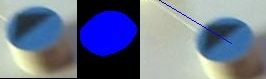
\includegraphics[width=40mm]{d1_i100_good_detection_example.jpg}
    \caption{Result on good detection}
\end{figure} 
In case of loose detection - detection where some addition non-robot region is 
misleadingly detected as a robot - detected direction perfectly matched the 
actual direction due to algorithms ability to filter noisy detections. 
\begin{figure}[h]
    \centering
    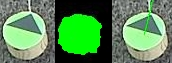
\includegraphics[width=40mm]{d2_i32_loose_detection_example.jpg}
    \caption{Result on loose detection}
\end{figure} 
In case of under-detection - detection where some parts of the image 
representing the robot where omitted - detected direction was skewed on the 
side opposite (from the axis matching the actual robot's direction) to the 
misdirected fragment of the robot. Error was proportional to the error of 
under-detected area of the robot. 
\begin{figure}[h]
    \centering
    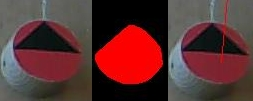
\includegraphics[width=40mm]{d4_i66_bad_detection_example.jpg}
    \caption{Result on under-detection detection}
\end{figure} 

\subsection{Tracking of the robots}
Tracing robots, as long as they were detected was trivial and worked as good as 
detection of the robots.
\begin{figure}[h]
    \centering
    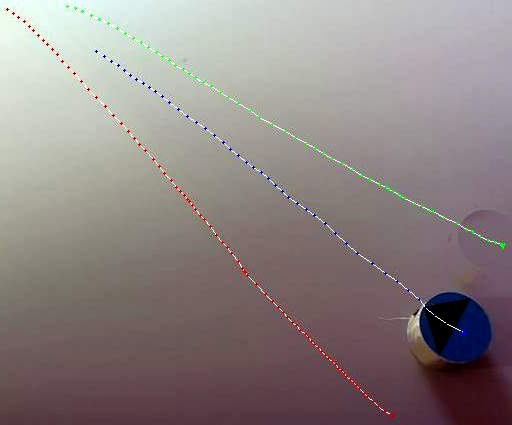
\includegraphics[width=40mm]{d1_trace.jpg}
    \caption{Trace of data set 1}
\end{figure} 


\section{Discussion}
Overall performance of the algorithm can be evaluated as good. It operates 
under little or no simplifying assumptions.
Robot detection could be improved [WRITE PLEASE HOW]
Another way how to improve the detection of the robots could be utilisation of 
second order spatial statistics of the robot images. Using such approach might 
give good results combined with our current approach.
Direction detection could be improved by making it less dependent on detection 
of the robots. It could be achieved by performing local search near the regions 
detected as robots. Such approach would improve accuracy of the directions 
detected, however it would make algorithm much slower. 
Another possible direction of development could be shape analysis - currently 
algorithms utilise only image's colour statistics due to limited information 
about the scale of the images and the possible placements of the camera. 


\section{Code}
the new Matlab code that you developed for this assignment. Do not
include code that you downloaded from the course web pages. Any other code
that you downloaded should be recorded in the report, but does not need to
be included in the appendix.

\end{document}
